
% !Mode:: "TeX:UTF-8" (encoding info for WinEdt)
\section{notes confidentielles}\label{Privatnotizen}
L'intégration des textes confidentiels dans le texte de la consultation. Einbindung vertraulicher Texte in den Konsultationseintrag. Ce plugin est une partie de la distribution standard.


Parfois on doit introduire des remarques dans un dossier électronique qu'on n'aimerait ni faire voir par d'autres collaborateurs ni exporter lors d'un transfert de dossier(par ex. des informations concernant des tiers). 
Ce plugin permet de faire des \textit{notes confidentielles}: S'il est installé on trouve lors qu'on clique la touche droite de la souris dans la fenêtre des consultations dans le menu contextuel une rubrique \textit{note}  :

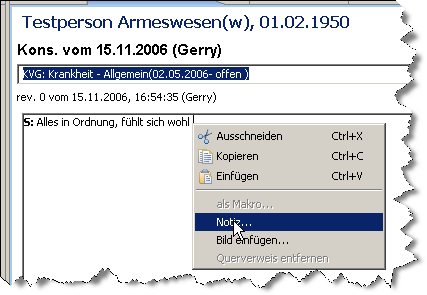
\includegraphics[width=3in]{images/notiz1.png}
% notiz1.png: 427x295 pixel, 96dpi, 11.30x7.80 cm, bb=0 0 320 221

SI vous cliquez sur note vous pouvez introduire un texte :

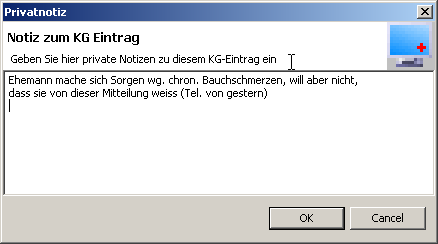
\includegraphics[width=3in]{images/notiz2.png}
% notiz2.png: 438x244 pixel, 96dpi, 11.59x6.46 cm, bb=0 0 328 183

Après avoir cliqué sur \textit{OK} une référence de \textit{note} indiquera la présence de cette note:

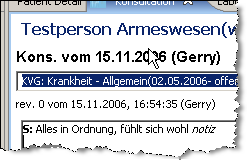
\includegraphics[width=3in]{images/notiz3.png}
% notiz3.png: 247x160 pixel, 96dpi, 6.53x4.23 cm, bb=0 0 185 120

En cliquant sur la référence, la fenêtre contenant la note s'ouvrira. Si un autre utilisateur s'est identifié aucune référence se montre.

Lors de l'exportation ou de l'impression du dossier toutes ces notes sont ignorées.


